\section{Methods}
\label{sec:methods}
\sksglenoid currently implements two 3D methods; the two-plane method described by Ganapathi et al. \cite{PMID:20933439} and the 3D corrected 
Friedman method described by Budge et al. \cite{BUDGE2011577}. \sksglenoid also implements two
2D methods; Friedman's method \cite{PMID:1522089} and the vault method described by Matsumura et al. \cite{PMID:24618285}. Each implementation can be accessed by via a command line application which takes as 
input a file describing the anatomical position of the required landmark points.

\begin{figure}
        \begin{center}
                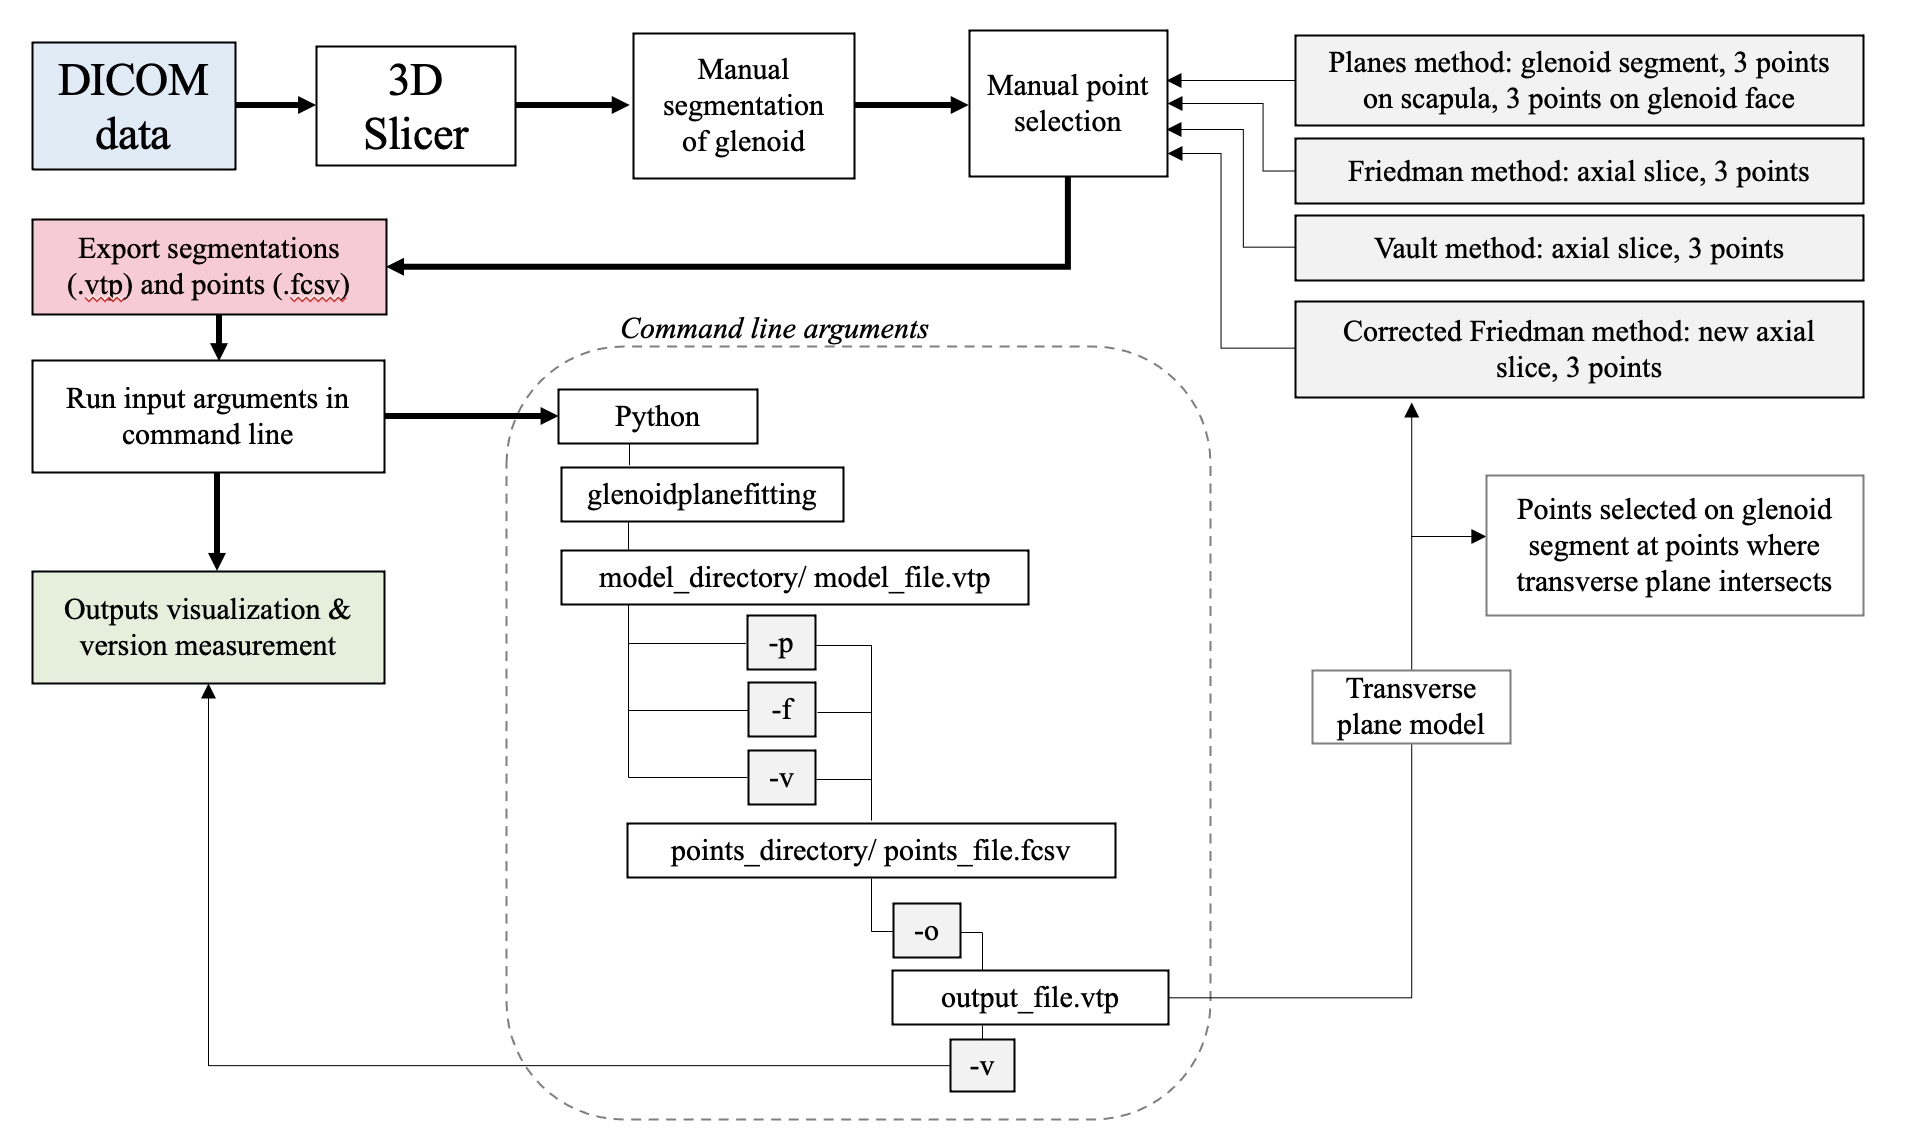
\includegraphics[width=0.85\linewidth]{figures/workflow.png}
                        \caption{\label{fig:workflow}A workflow diagram describing the current workflow. Relevant landmarks 
			are currently identified using 3DSlicer and passed to \sksglenoid via the command line.}
        \end{center}
\end{figure}

\sksglenoid currently requires these landmarks to be manually defined. We performed segmentation 
and landmark annotation using 3DSlicer \cite{Kikinis2014} on 10 patients and processed
the resulting 
segmentation using \sksglenoidns.

The selection of the different landmark points for each method and calculations of version measurements were done as follows. For the two-plane method, 3 points were chosen for each plane. For the glenoid fossa plane the points selected were near the rim, one at the superior pole of the glenoid and two on the lower third of the glenoid anteriorly and posteriorly.  For the scapula plane, the 3 points included one at the center of the glenoid, another at the medial border of the scapula where the scapular spine intersects the scapular body, and a third at the inferior tip of the scapula. The glenoid version was then calculated as the angle between the plane of the glenoid fossa and the plane of the scapula. 
\begin{figure}
        \begin{center}
                \begin{subfigure}[b]{0.31\linewidth}
			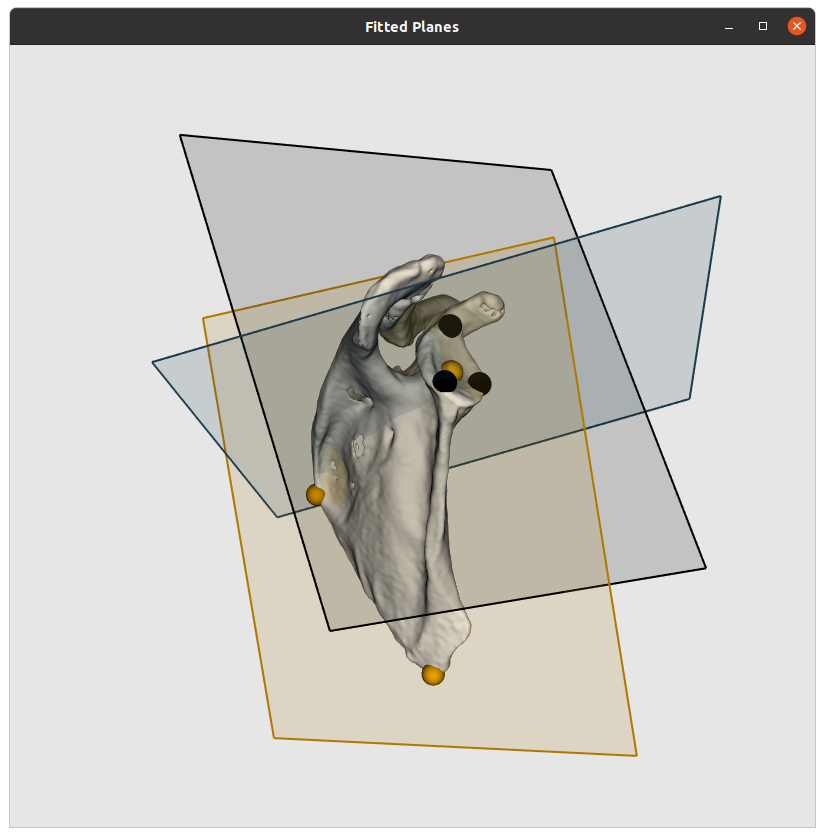
\includegraphics[width=\linewidth]{figures/planes_vis.png}
			\caption{\label{fig:visplanes}Two Plane Method}
		\end{subfigure}	
                \begin{subfigure}[b]{0.28\linewidth}
			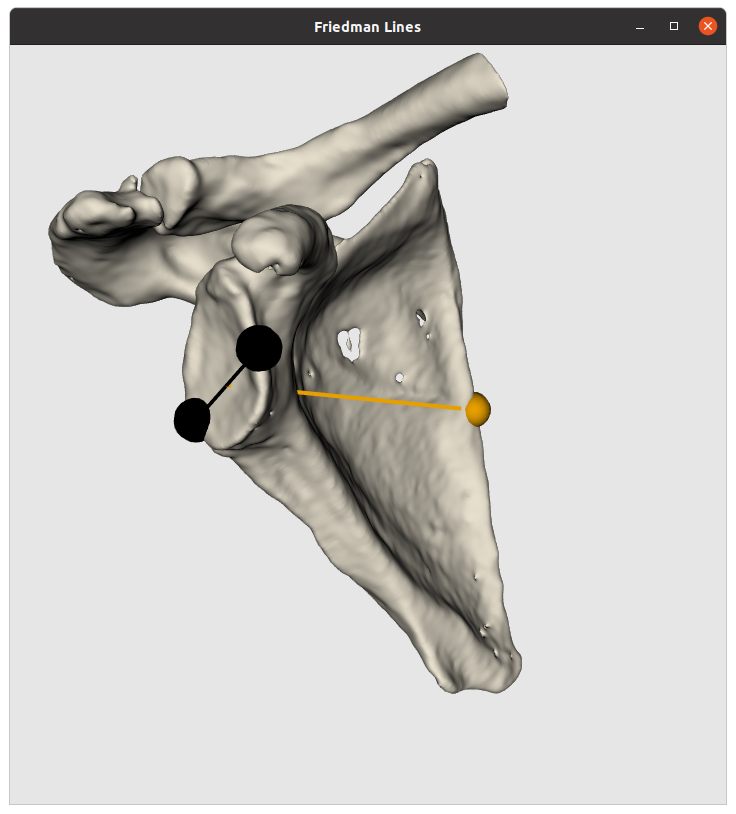
\includegraphics[width=\linewidth]{figures/friedman_vis.png}
			\caption{\label{fig:visfried}Friedman Method}
		\end{subfigure}	
                \begin{subfigure}[b]{0.31\linewidth}
			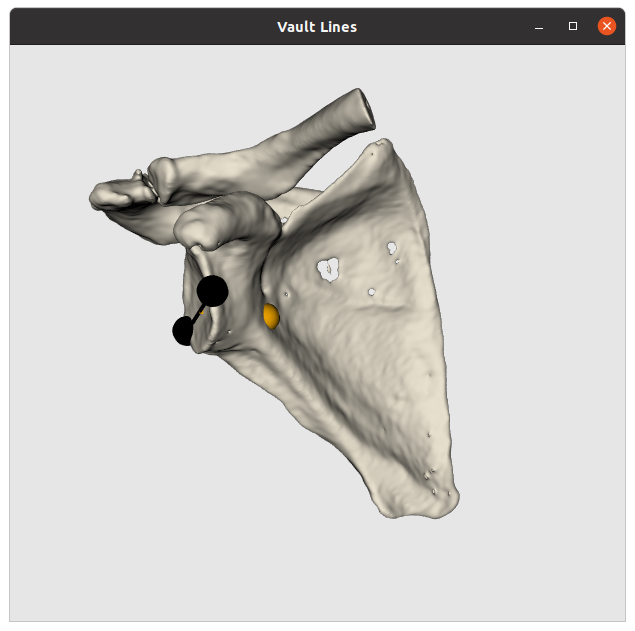
\includegraphics[width=\linewidth]{figures/vault_vis.png}
			\caption{\label{fig:visvault}Vault Method}
		\end{subfigure}	
	\end{center}
	\caption{\label{fig:visualisations}Visualisations of the 2 plane, Friedman and Vault methods. By default uses the colour blind friendly palette defined by Wong\cite{bang2011}}
\end{figure}

For the Friedman and vault method both 3 points were chosen to form 2 lines. Both require the same two points at the edges of the glenoid fossa anteriorly and posteriorly. For the Friedman method the third point was selected at the tip of the scapula, while for the vault method it was at the tip of the scapular vault. Slice choice is important and in this case was selected as the axial slice at which the coracoid process is no longer visible. The Friedman line was formed with the medial point on the scapula and the midpoint between the glenoid fossa points, while the vault line was formed with the tip of the scapular vault and the same midpoint. The second line was formed across the glenoid fossa in both methods The version was then calculated as the angle between the two lines.

The corrected Friedman method require the same anatomical landmark points as the conventional Friedman method, but on a corrected axial plane. This plane should be perpendicular to the scapular plane and was formed by selecting 3 different points. The 3 points included the inferior tip of the scapula, the center of the glenoid surface, and the medial pole of the scapula. This new transverse scapular plane was used to generate a new 2D image slice on which the same Friedman landmark points were selected.


Statistical analysis was performed using GraphPad Prism software version 8.0 for
Mac \footnote{GraphPad Software, San Diego, CA, USA}. The mean and standard deviation of 
each method was calculated and compared. Pearson’s correlation coefficient was 
determined between the commercial software and each method. 
A repeated measures ANOVA was performed to determine any significant differences
in version measurements between the methods. Significance level for all analyses was set at 0.05.
